\section{Classification of covariance matrices for SSVEP}
\label{sec:classofcov}

\changes{

\subsection{Fundamentals of classification}
\label{subsec:fund_class}

Given labelled samples $\x_i$ drawn from two classes or populations (positive and negative), a simple classification algorithm consists in assigning a previously unseen sample to the class with closer mean[ref: fig].
This implies a computation of means of classes and a measure of distances from the means. 
Assuming that the samples are embedded into a dot product space (i.e. with Euclidean geometry), the means can be computed as:

\begin{equation}
c_{+} = \frac{1}{m_{+}} \sum_{ \left\lbrace i|y_i=+1 \right\rbrace } \x_i,
\label{eq:mean_eucl1}
\end{equation}

\begin{equation}
c_{-} = \frac{1}{m_{-}} \sum_{ \left\lbrace i|y_i=-1 \right\rbrace } \x_i,
\label{eq:mean_eucl2}
\end{equation}
where $y_i \in \left\lbrace +1, -1 \right\rbrace$ is the label of the training sample $\x_i$, $m_{+}$ and $m_{-}$ the number of positive and negative samples respectively. 
An unseen sample $\x$ is unsigned to the class whose mean is the closest. 
This simple geometric classification framework is the founding principle of more complex algorithms such as supporting vector machines. }

\changes{
It can be formulated in terms of the dot product $\left\langle \cdot, \cdot \right\rangle$.
If $c:=(c_{+}+c_{-})/2$ is the point lying halfway between $c_{+}$ and $c_{-}$, and $w:=c_{+}-c_{-}$ the vector connecting $c_{+}$ to $c_{-}$, the class of the unseen sample $\x$ is determined by checking whether the vector $\x-c$ connecting $c$ to $x$ makes an angle $\alpha < \pi/2$ with $w$ [ref: fig].   
This is expressed as:

\begin{equation}
\begin{split}
y &= \mathrm{sgn} \left\langle (\x-c),w \right\rangle \\
  &= \mathrm{sgn} \left\langle (\x-(c_{+}+c_{-})/2),(c_{+}-c_{-}) \right\rangle \\
  &= \mathrm{sgn} (\left\langle \x,c_{+} \right\rangle - \left\langle \x,c_{-} \right\rangle + b)
\end{split}
\label{eq:classif1}
\end{equation}
where $\mathrm{sgn}$ is the sign function.
The offset $b$ vanishes if class means are equidistant to the origin \cite{scholkopf_learning_2001}.
Inserting \eqref{eq:mean_eucl1} and \eqref{eq:mean_eucl2} in \eqref{eq:classif1} yields:

\begin{equation}
y = \mathrm{sgn} \left( \frac{1}{m_{+}} \sum_{ \left\lbrace i|y_i=+1 \right\rbrace } \left\langle \x,x_i \right\rangle - \frac{1}{m_{-}} \sum_{ \left\lbrace i|y_i=-1 \right\rbrace } \left\langle \x,\x_i \right\rangle + b \right) .
\label{eq:classif2}
\end{equation}
Classifier \eqref{eq:classif2} can be generalized as:

\begin{equation}
y = \mathrm{sgn} \left( \sum_{i=1}^{m} y_i \alpha_i \dist(\x,\x_i) + b \right) ,
\label{eq:classif_gen}
\end{equation}
where $\alpha_i$ is the weight of the training sample $x_i$ and $\dist(\cdot, \cdot)$ a distance, a divergence of a kernel. 
In the case of two classes in the dot product space where all samples have the same weight, $y_i \in \left\lbrace +1, -1 \right\rbrace$, $\alpha = 1/m$ and $\dist(\cdot, \cdot) = \left\langle \cdot, \cdot \right\rangle$. 
}

\changes{
Expression~\eqref{eq:classif_gen} corresponds to the decision function used in hyperplane classifiers \cite{scholkopf_learning_2001}. 
This shows that even more complex classifiers rely on the calculations of class means (or centers) and their distances to individual samples.
This being shown, in this article we focus on the simple classification approach of assigning a previously unseen sample to the class with closest mean.
}

\changes{
In machine learning algorithms, samples are represented by their features which are determined through a feature extraction and selection process.
In this work, samples are represented by their covariance matrices. Therefore means of classes and distances to mean will be means of covariance matrices and distance between them.
}

\subsection{Means of Covariance matrices}
\label{subsec:mean}

\changes{
Consider a multivariate variable $\X \in \Re^{\dc \times \dt}$ where $\dc$ is the number of variables and $\dt$ the number of samples, with $C > N $, the covariance matrix of the centered variable $\X$ can be estimated as:

\begin{equation}
\cov{} = \frac{1}{\dt} \X \X^\intercal
\end{equation}
and is symmetric positive definite (SPD).
The properties of SPD matrices constrain them to a convex cone:

\begin{enumerate}
[label=(\roman*)]
\item Symmetry: \tab $\P = \P^\intercal$ ,
\item Positive definiteness: \tab $\x^\intercal \P \x > 0, \forall x \in \Re^{\dc} \backslash 0$ ,
\item Strict positivity of diagonal element: \tab $\P(i,j) > 0 | i=j, \forall i,j \in \left\lbrace 1, \dots, \dc \right\rbrace$ i.e. positive variance ,
\item Cauchy-Schwarz inequalities: \tab $|\P(i,j)| \leq (\P(i,i) \P(j,j))^{1/2}, \forall i,j \in \left\lbrace 1, \dots, \dc \right\rbrace$ .
\end{enumerate}
}

\changes{
The mean of SPD matrices can be computed as a center of mass modeled on Euclidean geometry:}
given a set of covariance matrices $\{\P_\nb\}_{\nb=1,\dots,\Nb}$,
the center of mass $\Pm$ of the set, is a covariance matrix that minimizes the sum of the squared distances to matrices $\P_\nb$:

\begin{equation}
	\label{eq:mean}
	\Pm = \Rm(\P_1, \dots, \P_\Nb) = \argmin_{\P \in \Ma} \sum_{\nb=1}^{\Nb} \dist^2(\P_\nb,\P) \ ,
\end{equation}
where $\dist(\cdot,\cdot)$ is a measure of distance between two matrices. \changes{Practically, $\dist(\cdot,\cdot)$ can either be a distance or a divergence.}
\changes{
In the literature, this  mean is at times designated as the \emph{Frechet mean}, \emph{Cartan mean}, or \emph{Karcher mean} \footnote{This appellation has been recently criticized by Karcher himself \cite{karcher_riemannian_2014}} \cite{lim_matrix_2012}.
Cartan \cite{cartan_groupes_1929} had shown that a unique solution to \eqref{eq:mean} exists if all $\P_\nb$ lie in a convex ball \citep[section 16 of][]{cartan_groupes_1929}. This applies also to closed convex cones.}

\changes{Depending on the divergence or distance used, several means can be defined from \eqref{eq:mean}. Those considered in this study are presented in the next lines and summarized in Table~\ref{tab:dist}.}

\changes{

\subsubsection{Distance and divergence}
Divergences and distances are measures of dissimilarity between two points in a space.
Here the Riemannian space will be considered.
A distance function $\dist:\GenMa \times \GenMa \rightarrow \Re^+$ has the following properties for all $\P_1, \P_2,\P_3 \in \GenMa$:

\begin{enumerate}
[label=(\roman*)]
\item Non-negativity: \tab $\dist(\P_1, \P_2) \geq 0$ ,
\item Identity: \tab $\dist(\P_1, \P_2) = 0 \ \ \mathrm{iff} \ \ \P_1 = \P_2$ ,
\item Symmetry: \tab $\dist(\P_1, \P_2) = \dist(\P_2, \P_1)$ ,
\item Triangular inequality:  \tab $\dist(\P_1, \P_3) \leq \dist(\P_1, \P_2) + \dist(\P_2, \P_3)$ .
\end{enumerate}
Divergences are very similar to distances with the difference that properties (iii) and (iv) do not have to be satisfied. 
In the context of covariance matrices, divergences and distances should both induce a Riemannian metric on the manifold of SPD matrices. 
}
\changes{

\subsubsection{Euclidean distance}
The Euclidean distance between two matrices is represented by the \emph{Frobenius norm} of their difference:

\begin{equation}
\distF(\P_1, \P_2) = \lVert \P_1-\P_2 \rVert _F
\label{eq:dist_eucl}
\end{equation}
In \eqref{eq:mean}, this yields the arithmetic mean:

\begin{equation}
\PmE = \frac{1}{\Nb}\sum_{\nb=1}^{\Nb} \P_\nb
\label{eq:mean_arithmetic}
\end{equation}
The arithmetic mean is drown from a family of power means ($\P_{t|t = 1}$) [TODO: reference Lim2012]:

\begin{equation}
\P_t = \left( \frac{1}{\Nb}\sum_{\nb=1}^{\Nb} \P_\nb^t \right)^{\frac{1}{t}}, \ t \in [-1,+1].
\label{eq:mean_power}
\end{equation}
From the same family can be drawn the \emph{geometric mean} ($\P_{t|t \rightarrow 0}$) and the \emph{harmonic mean} ($\P_{t|t = -1}$).
}
\changes{
We consider the arithmetic mean $\PmE$, as a baseline. 
This averaging of covariance is usually not adequate in the space of SPD matrices for two main reasons. 
Firstly, the Euclidean distance and averaging do not grantee invariance under inversion: a matrix and its inverse are supposed to be at the same distance from the identity matrix. 
Secondly, the Euclidean averaging of covariance SPD leads to a \emph{swelling effect}: the determinant of the arithmetic mean of SPD matrices can be larger than the determinant of its individual components.
And since the determinant of a covariance matrix is a direct measure of the dispersion of the multivariate variable, the swelling effect introduces a large distortion of the data dispersion \cite{arsigny_geometric_2007}.
For these reasons, other means that adapt to the geometry of convex cone of SPD matrices are used. 
} 
\changes{

ON DIRAIT QU'ICI, UN PARAGRAPHE A DISPARU !

\[
 \metric_\P: T_\P\GenMa\times T_\P\GenMa \rightarrow \Re \]
$\metric$ is a function that assigns, for each point $\P \in \GenMa$, an inner product in the tangent space $T_\P\GenMa$  .
The Riemannian metric allows us to compute the length of vectors or distance between two point on the tangent space, and through appropriate mapping \cite{pennec_riemannian_2006}, the length of the corresponding \emph{geodesic} (i.e. the shortest curve connecting two point) on the manifold $\GenMa$.
The \emph{affine-invariant distance} is the distance between two points of a Riemannian  manifold endowed with an invariant Riemannian metric:
\begin{equation}
\begin{split}
g_{\P}(\S_1, \S_2) & = \left\langle \S_1|\S_2 \right\rangle_\P \\
 & = \left\langle  \P^{-\frac{1}{2}} \S_1  \P^{-\frac{1}{2}} |  \P^{-\frac{1}{2}} \S_2  \P^{-\frac{1}{2}} \right\rangle_\eye\\
 & = \mathrm{trace} \left( \P^{-\frac{1}{2}} \S_1 \P^{-1} \S_2 \P^{-\frac{1}{2}} \right) ,
\end{split}
\label{eq:metric-riemann}
\end{equation}
where $\eye$ is the identity matrix. 
The inner product of the tangent vectors $\S_1$ and $\S_2$ at $\P$ is invariant by the action of $\P^{-\frac{1}{2}}$ transformation.
The affine-invariant Riemannian distance is defined as:
\begin{equation}
\distAIRM(\P_1, \P_2) = \lVert \log(\P_1^{-1}\P_2) \rVert_F = \left[ \sum_{\chI=1}^{\dc} \log^2 \lambda_\chI \right]^{1/2},
\label{eq:dist_air}
\end{equation}
where $\lambda_\chI$, $\chI = 1, \dots, \dc$, are the eigenvalues of $\P_1^{-1}\P_2$.
}

\changes{
Inserting \eqref{eq:dist_air} in \eqref{eq:mean} yields the mean $\PmAIRM$ associated to the affine-invariant metric. 
It is the solution to 
\begin{equation}
\sum_{\nb=1}^\Nb \log(\PmAIRM^{-1/2} \P_\nb \PmAIRM^{-1/2})=0
\label{mean_air}
\end{equation}
It has no close form solution and can be solved iteratively through a gradient descent algorithm \cite{letcher_principal_2004}. 
} 

\changes{
These distance and mean are invariant to affine transformations. 
Some of these invariances are particularly important to preserve the geometric topology of the Riemannian manifold of SDP matrices. Let $f$ be an affine-invariant function defined on $\GenMa$ (e.g. distance or mean),
\begin{enumerate}[label=(\roman*)]
\item \emph{Invariance under congruent transformation}
\begin{equation}
f(\P_1, \P_2) = f(\P \P_1 \P^\intercal, \P \P_2 \P^\intercal)
\label{eq:invar_congr}
\end{equation}
\item \emph{Invariance under inversion}
\begin{equation}
f(\P,\eye) = f(\P^{-1},\eye)
\label{eq:invar_invers}
\end{equation}
implying
\begin{equation}
f(\P_1,\P_2) = f(\P_1^{-1},\P_2^{-1})
\label{eq:invar_invers2}
\end{equation}
\end{enumerate}
Another interesting property of the affine-invariant metric is its invariance to left- and right-multiplication by a positive matrix.
\begin{equation}
f(\P_1, \P_2) = f(\P \P_1, \P \P_2) = f(\P_1 \P, \P_2 \P)
\label{eq:invar_mult}
\end{equation}
}  

\changes{    
\subsubsection{Log-Euclidean}
The Log-Euclidean is another distance that takes into consideration the topology of Riemannian manifolds. 
It was introduced by Arsigny et al. to alleviate the complexity involved in the computation of the affine-invariant distance and its related mean \citep{arsigny_geometric_2007}.
The mean associated to the Log-Euclidean distance corresponds to an arithmetic mean in the domain of matrix algorithm.  
The distance between two SPD matrices is expressed as
\begin{equation}
\distLE(\P_1, \P_2) = \lVert \log(\P_1)-\log(\P_2) \rVert_F ,
\label{eq:dist_LE}
\end{equation}
and its associated mean is defined explicitly:
\begin{equation}
\PmLE = \exp \left(\sum_{\nb=1}^{\Nb} \log(\P_\nb) \right) .
\label{eq:mean_LE}
\end{equation}
Unlike the affine-invariant mean, the Log-Euclidean mean as a closed form expression which gives it a large computational advantage. 
Moreover, the obtained mean is, to a large extent, similar to the affine-invariant mean:
\begin{enumerate}[label=(\roman*)]
\item they have the same determinants which correspond to the geometric mean of the determinants of their building matrices: \[ |\PmLE| = |\PmAIRM| = \prod_{\nb=1}^{\Nb} (|\P_\nb|)^{1/\Nb} = \exp(\frac{1}{\Nb}\sum_{\nb=1}^{\Nb}\log(|\P_\nb|)) \] ;
\item they are often equal in value, if not, $\mathrm{trace}(\PmLE) > \mathrm{trace}(\PmAIRM)$ ;
\item Log-Euclidean mean has properties close to affine-invariance (i.e. similarity-invariance instead of congruent-invariance).
\end{enumerate}
}
\changes{
\subsubsection{Bregman divergences}
Divergences have been considered for the computation of mean in applications of clustering and classification of SPD matrices due to the fact that they induce a Riemannian metric given by \eqref{eq:metric-riemann}. 
Consider a strictly convex and differentiable function $f: \Re \rightarrow \Re$; then $f(x) \geq f(y) + f'(y)(x-y)$ and $f(x) = f(y) + f'(y)(x-y) \Leftrightarrow x = y$ for all $x,y \in \Re$.  
The Bregman divergence, \citep[introduced by Bregman in][]{bregman_relaxation_1967} is the difference between the left and right sides of the inequality:
\begin{equation}
\divB{f}(x,y) = f(x)-f(y)-f'(y)(x-y).
\label{eq:bregman-div}
\end{equation} 
$f$ is called a \emph{seed function}.
It is shown that $\divB{f}$ verifies the non-negativity and the identity properties. When the seed function is quadratic, it can also be symmetric. 
There is another set of properties that $\divB{f}$ verifies, reported in \cite{bregman_relaxation_1967}.
Geometrically, the Bregman divergence can be seen as the measure of the difference between $f(x)$ and its representation on the plane tangent to $f$ at $y$ as illustrated in Fig.~\ref{fig:bregman-projection}.
\begin{figure}[ht!]
\centering
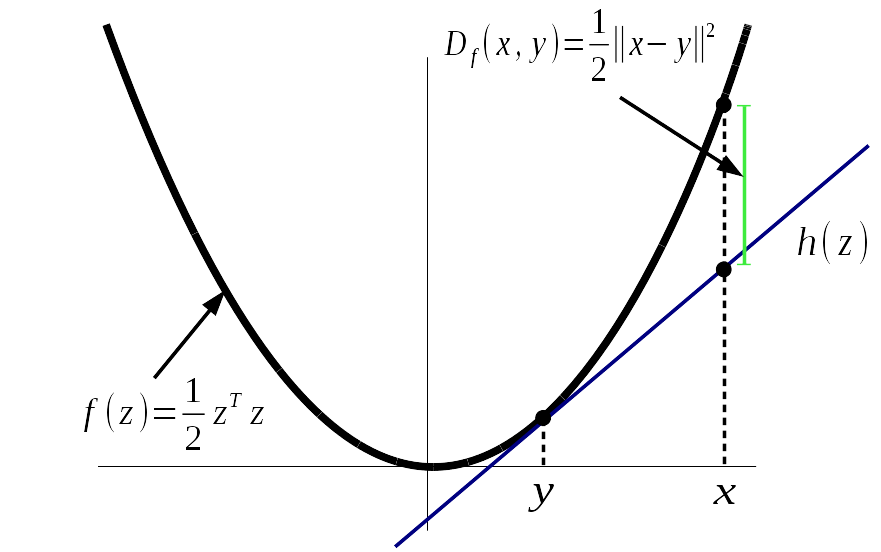
\includegraphics[width=0.6\columnwidth]{Figures/bregman_projection}
\caption{Geometry of the Bregman divergence with the seed function $f(z)=\frac{1}{2}z^\intercal z$. $h(z)$ is a hyperplane tangent to $f(z)$ at $y$. While it accurately represent $f(y)$, it underestimate $f(x)$. The Bregman divergence measure how much the representation of $f(x)$ on $h(z)$ \emph{diverges} from $f(x)$ (in green).}
\label{fig:bregman-projection}
\end{figure}
}

\changes{
The scalar divergence can be directly adapted to SPD matrices as:
\begin{equation}
\divB{f}(\P_1,\P_2) = \varphi(\P_1) - \varphi(\P_2) - \varphi'(\P_2)(\P_1 - \P_2),
\end{equation}
where the seed function $f$ is combined with a function $\lambda: \GenMa \rightarrow \Re^\dc$ that maps an SPD matrix to a vector containing its eigenvalues: $\varphi = f \circ \lambda$.\\
Or, $\lambda$ can be the trace function, $\lambda: \GenMa \rightarrow \Re$ that maps an SPD matrix to its trace.
For convenience, $f \circ \lambda$ will be referred to as $f(X)$ or $f(\P)$. 
}
\changes{
Depending on the seed function used, various divergences can be defined defined from the Bregman divergence.

%- Squared Norm -> Euclidean divergence = Frobenious Norm (Dhillon 2007)
\\ \\ \textbf{Euclidean divergence} \\
The Frobenius norm is also a Bregman divergence in disguise. 
It is obtained when the seed function  is the squared norm $f(x) = \frac{1}{2} \lVert x \rVert_2^2$ \cite{dhillon_matrix_2007}:
\begin{equation}
\divB{E}(\P_1, \P_2) = \lVert \P_1-\P_2 \rVert _F
\label{eq:div-eucl}
\end{equation}
The Euclidean mean of SPD matrices correspond to their arithmetic mean \eqref{eq:mean_arithmetic}.
%\begin{equation}
%\PmE = \frac{1}{\Nb}\sum_{\nb=1}^{\Nb} \P_\nb
%\label{eq:mean-eucl}
%\end{equation} 

%- Shannon Entropy -> KL div (Nilson 2009)
\\ \\ \textbf{Kullback-Leibler divergence} \\
Using the \emph{Shannon entropy} $f(x) = \sum_\nb x_\nb \log x_\nb$ yields the \emph{Kullback-Leibler} divergence \cite{nielsen_sided_2009}.
It is also known as the \emph{relative entropy} or \emph{discrimination information}.
The Kullback-Leibler divergence of SPD matrices $\P_1, \P_2 \in \GenMa^C$ is given by:
\begin{equation}
\divB{KL}(\P_1, \P_2) = \frac{1}{2} \log \frac{\det(\P_2)}{\det(\P_1)} + \tr(\P_2 \P_1) - \dc
\label{eq:div-kl}
\end{equation}
The mean of SPD matrices induced by the Kullback-Leibler divergence is calculated iteratively \cite{chebbi_means_2012}. 
%- logarithmic barrier function -> Log det divergence (Dhillon 2007)
\\ \\ \textbf{Log-det divergence} \\
Another function often used in Bregman divergences of symmetric matrices is the \emph{logarithmic barrier} \cite{chebbi_means_2012,dhillon_matrix_2007,cherian_efficient_2011,sra_positive_2016}
\[ f(x) = -log(x) \rightarrow f(\P) = -\log \det(\P) \] 
The corresponding divergence is called the \emph{log-det} divergence and is given by \cite{chebbi_means_2012}:
\begin{equation}
\divB{ld}(\P_1,\P_2) = \left\langle \P_1, \P_2^{-1} \right\rangle - \log \det(\P_1 \P_2^{-1})-\dc
\label{eq:div-log-det}
\end{equation}
}
\changes{
The asymmetry of divergences result in the concept of right- and left-sided mean:
\[ \divB{f}(\P_1,\P_2) \neq \divB{f}(\P_2,\P_1) \Rightarrow \argmin_{\P \in \Ma} \sum_{\nb=1}^{\Nb} \dist^2(\P_\nb,\P) \neq \argmin_{\P \in \Ma} \sum_{\nb=1}^{\Nb} \dist^2(\P, \P_\nb) \]
It is usually sufficient to consider a single sided divergence. 
In this work right-sided divergence and mean are used.
In some cases however, the asymmetry can be undesirable. This has led to the symmetrization of some Bregman divergences.
Often the symmetrization consist in an averaging of left- and right-sided divergence [todo: reference].

\\ \\ \textbf{S-divergence}\\
An example of a symmetric divergence is the S-divergence. 
It is obtained from the \emph{Jensen-Shannon} divergence which is a symmetrized Bregman divergence:
\begin{equation}
\begin{split}
\divB{J-S}(\P_1, \P_2) & = \frac{1}{2} \left( \divB{f}(\P_1,\frac{\P_1+\P_2}{2}) + \divB(\frac{\P_1+\P_2}{2},\P_2) \right) \\
 & = \frac{1}{2} \left( \tr f(\P_1) + \tr f(\P_2) \right) - \tr f(\frac{\P_1+\P_2}{2})
\end{split} 
\label{eq:div-js}
\end{equation}
The S-divergence is obtained by using the logarithmic barrier function for the positive definite cone $f(\P)=-\log \det(\P)$ as seed in $\divB{S-J}$ \cite{sra_positive_2016}:
\begin{equation}
\div{S}(\P_1,\P_2) = \log \det(\frac{\P_1+\P_2}{2}) - \frac{1}{2}\log \det(\P_1 \P_2)
\label{eq:div-s}
\end{equation}  
Despite its symmetry, S-Divergence is not a metric. It does not satisfy the triangular inequality criterion. 
However, its square root has been shown to be a distance \cite{sra_positive_2016}.
}

\changes{
Other symmetric divergences can be obtained in the same fashion; for instance the \emph{Jeffreys divergence} which is a symmetrized Kullback-Leibler divergence: $\divB{J}(\P_1, \P_2) = \divB{KL}(\P_1, \P_2) + \divB{KL}(\P_2, \P_1)$ \cite{sra_positive_2016}.
}

\changes{
Another family of divergence is defined when the right- and left-sided divergence are mixed in a weighted manner.
One such family is the \emph{$\alpha$-divergence} \cite{nielsen_clustering_2014}.
\\ \\ \textbf{Log-det $\alpha$-divergence}\\
In this work, the $\alpha$-divergence used is defined by \cite{chebbi_means_2012}:
\begin{equation}
\divB{f}^\alpha(\P_1,\P_2) = \frac{4}{1-\alpha^2}\left[ \frac{1-\alpha}{2} f(\P_1) + \frac{1+\alpha}{2}f(\P_2) - f \left( \frac{1-\alpha}{2}\P_1 + \frac{1+\alpha}{2}\P_2 \right) \right], \alpha^2 \neq 1
\label{eq:div-alpha}
\end{equation}
$\divB{f}^\alpha$ can be expressed in terms of Bregman divergence as:
\begin{equation}
\divB{f}^\alpha = \frac{4}{1-\alpha^2}\left[\frac{1-\alpha}{2}\divB{f}\left(\P_1, \frac{1-\alpha}{2}\P_1+\frac{1+\alpha}{2}\P_2\right) + \frac{1+\alpha}{2}\divB{f}\left(\P_2, \frac{1-\alpha}{2}\P_1 + \frac{1+\alpha}{2} \P_2 \right)\right], \alpha^2 \neq 1
\label{eq:div-alpha2}
\end{equation}
$\alpha$-divergences at $\alpha = \pm 1$ are obtained through the limit values $\lim_{\alpha \rightarrow \pm 1}\divB{f}^\alpha$.\\
Using the logarithmic-barrier function yields:
\begin{equation}
\begin{split}
\divB{LD}^\alpha(\P_1,\P_2) &= \frac{4}{1-\alpha^2}\log \det \left(\frac{1-\alpha}{2}\left(\P_1 \P_2^{-1}\right)^{\frac{1+\alpha}{2}}+\frac{1+\alpha}{2}\left(\P_2 \P_1^{-1}\right)^{\frac{1-\alpha}{2}}\right), \quad -1 < \alpha < 1 \\
\divB{LD}^{1}(\P_1,\P_2) &= \tr \left( \P_2^{-1}\P_1-\eye \right) - \log \det \left(\P_2^{-1}\P_1 \right)\\
\divB{LD}^{-1}(\P_1,\P_2) &= \tr \left(\P_1^{-1}\P_2-\eye \right) - \log \det \left(\P_1^{-1}\P_2 \right) .
\end{split}
\label{eq:div-log-det-alpha}
\end{equation}   
$\divB{LD}^{1}$ and $\divB{LD}^{-1}$ are right- and left-sided Bregman divergences respectively.
At $\alpha=0$, the log-det $\alpha$ divergence yields a symmetric divergence corresponding to the \emph{Bhattacharrya} divergence \cite{chebbi_means_2012,sra_positive_2016}. 
}

%\subsubsection{log-det alpha divergence}
%\subsubsection{Kullback Leibler divergence}
%\subsubsection{Bhattacharyya}
%\subsubsection{S-divergence}

\subsubsection{Wasserstein}

\begin{table}[h]
  \centering
  \begin{tabular}{ l | c | c | c |}
    \cline{2-4}
    & Distance/Divergence & Mean & References \rule[-5pt]{0pt}{18pt} \\ \hline
    \multicolumn{1}{|l|}{Euclidean} & $\distF(\P_1, \P_2) = \lVert \P_1-\P_2 \rVert _F$ & $\PmE = \frac{1}{\Nb}\sum_{\nb=1}^{\Nb} \P_\nb$ & \rule[-5pt]{0pt}{18pt} \\   
		 \multicolumn{1}{|l|}{Log-Euclidean} & $\distLE(\P_1, \P_2) = \lVert \log(\P_1)-\log(\P_2) \rVert_F$ & $\PmLE = \exp \left(\sum_{\nb=1}^{\Nb} \log(\P_\nb) \right) $ & \cite{arsigny_geometric_2007} 
		\rule[-5pt]{0pt}{18pt} \\    
     \multicolumn{1}{|l|}{Affine-invariant} & $\distAIRM(\P_1, \P_2) = \lVert \log(\P_1^{-1}\P_2) \rVert_F$ & Algorithm 3 in \cite{fletcher_principal_2004}  & \cite{moakher_differential_2005,letcher_principal_2004} 
		\rule[-5pt]{0pt}{18pt} \\	
	\multicolumn{1}{|l|}{Kullback-Leibler} & $\divB{KL}(\P_1, \P_2) = \frac{1}{2} \log \frac{\det(\P_2)}{\det(\P_1)} + \tr(\P_2 \P_1) - \dc$ & Algorithm 1 in \cite{chebbi_means_2012} & \cite{chebbi_means_2012,kang_composite_2009} \rule[-5pt]{0pt}{18pt} \\
	\multicolumn{1}{|l|}{S-divergence} & $\divB{S}(\P_1,\P_2) = \log \det(\frac{\P_1+\P_2}{2}) - \frac{1}{2}\log \det(\P_1 \P_2)$ &  Eq. (17-20) in \cite{cherian_efficient_2011} & \cite{sra_positive_2016,cherian_efficient_2011} \rule[-5pt]{0pt}{18pt} \\
    \multicolumn{1}{|l|}{$\alpha$-divergence} & $\divB{LD}^\alpha (\P_1, \P_2)$ from Eq.~\eqref{eq:div-log-det-alpha} & Algorithm 1 in \cite{chebbi_means_2012} & \cite{chebbi_means_2012} \rule[-5pt]{0pt}{18pt} \\ 
    \multicolumn{1}{|l|}{Bhattacharyya} & $\divB{B}(\P_1, \P_2)=\left( \log \frac{ \det \frac{1}{2} (\P_1+\P_2)}{(\det (\P_1)\det(\P_2))^{1/2}} \right)^{1/2}$ & Algorithm 1 in \cite{chebbi_means_2012} & \cite{nielsen_matrix_2012,chebbi_means_2012} \rule[-5pt]{0pt}{18pt} \\ 
    \multicolumn{1}{|l|}{Wasserstein} &  &  &  \rule[-5pt]{0pt}{18pt} \\ \hline
  \end{tabular}
  \caption{Distances, divergences and means considered in the experimental study.}
  \label{tab:dist}
\end{table}
\subsection{Minimum Distance to Mean classifier for SSVEP}
\label{subsec:mdm}
\changes{The considered classifier is described in section \ref{subsec:fund_class}. 
It is given the name \emph{Minimum Distance to Mean} or MDM, and was inspired from~\cite{barachant_multiclass_2012} where it is limited to Riemannian mean.
%The considered classifier is referred to as Minimum Distance to Mean (MDM), and is inspired from~\cite{barachant_multiclass_2012} where it is limited to Riemannian mean. 
Covariance matrices of EEG trials are classified based on their distance to the centers of the classes (i.e. means or centroids).
To embed frequency information in the covariance matrices, we use a construction of matrices proposed in~\cite{congedo_new_2013}.
%In a SSVEP experiment with $\dF$ stimulus blinking at $\dF$ different frequencies, 
Let $\X \in \Re^{\dc\times\dt}$ be an EEG trial measured on $\dc$ channels and $\dt$ samples in a SSVEP experiment with $\dF$ stimulus blinking at different frequencies.  
The covariance matrices are estimated from a modified version of the input signal $\X$: %as explained in~\cite{congedo_new_2013}
%%Let $X \in \Re^{p \times n}$ be the recorded data with $p$ the number of channels, and $n$ the number of sample per trial. 
%%The extended data are defined as:
%Let consider an experimental SSVEP setup with $\dF$ stimulus blinking at $\dF$ different frequencies. 
%It is a multiclass classification with $\dK=\dF+1$ classes: one class per stimulus and one resting state class.
%The covariance matrices are estimated from a modified version of the input signal $\X$: %as explained in~\cite{congedo_new_2013}
%Let $X \in \Re^{p \times n}$ be the recorded data with $p$ the number of channels, and $n$ the number of sample per trial. 
%The extended data are defined as:
\begin{equation}
	\X \in \Re^{\dc \times \dt} \rightarrow 	
	\begin{bmatrix}
		X_{\text{freq}_1}\\ \vdots \\ X_{\text{freq}_{\dF}} \\
	\end{bmatrix}
	\in \Re^{\dF\dc \times \dt} \ ,
	\label{eq:ext_data}
\end{equation}
where $X_{\text{freq}_\df}$ is the input signal $\X$ band-pass filtered around frequency $\text{freq}_\df$, $\df=1, \ldots, \dF$. Henceforth, all EEG signals will be considered as filtered and modified by Eq.~\eqref{eq:ext_data}.
The associated covariance matrix $\P \in \Re^{\dF\dc \times \dF\dc}$ is estimated using the Sch\"{a}fer skrinkage estimator \cite{schafer_shrinkage_2005}.

For SSVEP classification, $\dK = \dF + 1$ classes are considered: one class for each target frequency, and one for the resting state.
As described in Algorithm~\ref{alg:mdm}, from $\dT$ labelled training trials $ \left\{ \X_{\ti} \right\}_{\ti=1}^{\dT}$ recorded per subject, $\dK$ centers of classes $\Pm^{(\ci)}$ are estimated (step~\ref{op:class_center}). 
In this step, outliers matrices are removed to have a reliable mean estimation \cite{barachant2013riemannian}.
A new unlabeled test trial $\Y$ is predicted to belong to the class whose mean $\Pm^{(\ci)}$ is the closest to the trial covariance matrix, w.r.t. one of the distances from Table~\ref{tab:dist} (step~\ref{op:decision}).

\begin{algorithm}
\caption{Minimum Distance to Mean Classifier}
\label{alg:mdm}
	Inputs: $\X_{\ti} \in \Re^{\dF \dc\times\dt}$, for $\ti = 1, \ldots, \dT$, a set of labelled EEG trials. \\
	Inputs: $\setindex(\ci)$, a set of indices of trials belonging to class $\ci$. \\
	Input: $\Y \in \Re^{\dF \dc\times\dt}$, an unlabeled test EEG trial. \\
	Output: $\clout$, the predicted label of $\Y$.
	\begin{algorithmic}[1]
	\State Compute covariance matrices $\P_{\ti}$ of $\X_\ti$ 
	\State \textbf{for} $\ci$ = 1 \textbf{to} $\dK$ \textbf{do}
	\State \quad Compute center of class : $\Pm^{(\ci)}=\Rm(\P_{\ti}:\ti \in \setindex(\ci))$
	\label{op:class_center}
	\State \textbf{end}
	\State Compute covariance matrix $\P$ of $\Y$, and classify it : $\clout = \arg \min_{\ci} \dist(\P, \Pm^{(\ci)})$
	\label{op:decision}
	\State \textbf{return} $\clout$
	\end{algorithmic}
\end{algorithm}

%%%%%%%%%%%%%%%%%%%%%%%%%%%%%%%%%%%%%%%%%%%%%%%%%%%%%%%%%%%%%%%%%%%%%%%%%%%%%%%%

\section{Experimental Results}
\label{sec:expresults}
This section presents experimental results obtained applying Euclidean and Riemannian distances in SSVEP classification task. 
%The performances are compared with LDA. 
The first part of this section describes the data used and the second part provides the assessment of the classification for the considered distances and divergences. %classifications accuracies obtained. 

\subsection{SSVEP Dataset}
The experimental study is conducted on multichannel EEG signals recorded during an SSVEP-based BCI experiment~\cite{kalunga_hybrid_2014}.   
EEG are recorded on $\dc=$ 8 channels from 12 subjects.
The subjects are presented with $\dF=$ 3 visual target stimuli blinking respectively at 13Hz, 21Hz and 17Hz. %$\text{freq}=$
It is a $\dK=$ 4 classes setup combining $\dF=$ 3 stimulus classes and one resting class (no-SSVEP).
In a session, 32 trials are recorded: 8 for each visual stimulus and 8 for the resting class. 
The number of sessions recorded per subject varies from 2 to 5.
For each subject, a test set is made of 32 trials while the remaining trials (which might vary from 32 to 128) make up for the training set.

\subsection{Results and Discussion}

\changes{
Discuss the invariance to right- and left-multiplication by positive matrices. It brings a significanc advantage over Euclidean metrics, in terms of electrode placement and unforseen displacement in electrodes position, and can even alleviate anatomical differences.
}
\begin{figure}[h!]
\centering
\subfigure[]{
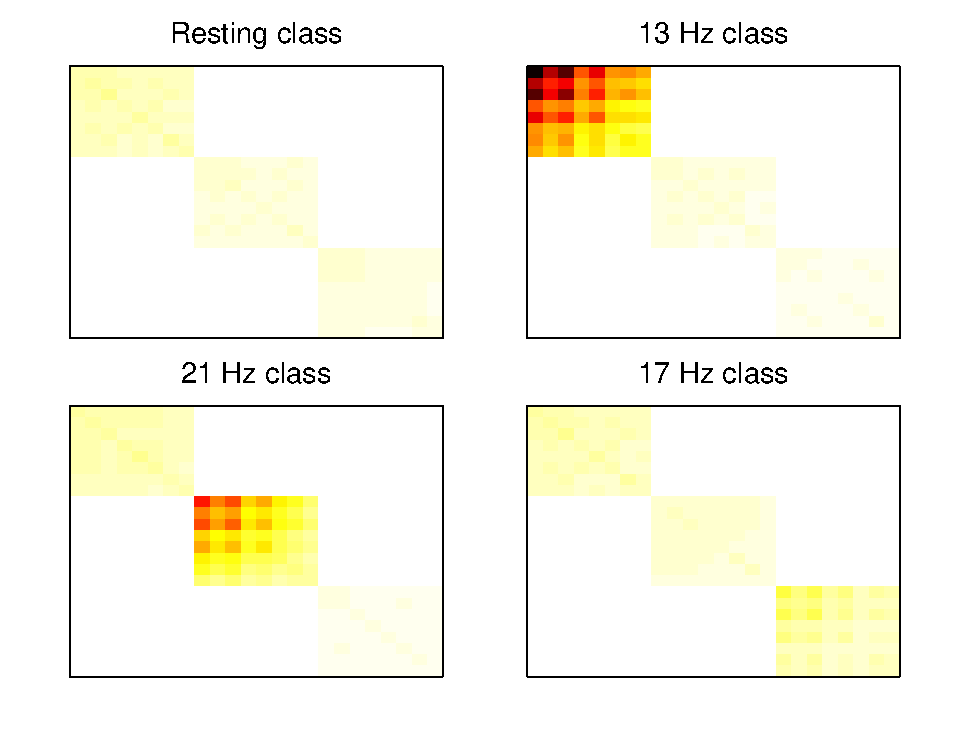
\includegraphics[width=0.47\textwidth]{Figures/covmat.eps}
\label{fig:covmat12}}
\subfigure[]{
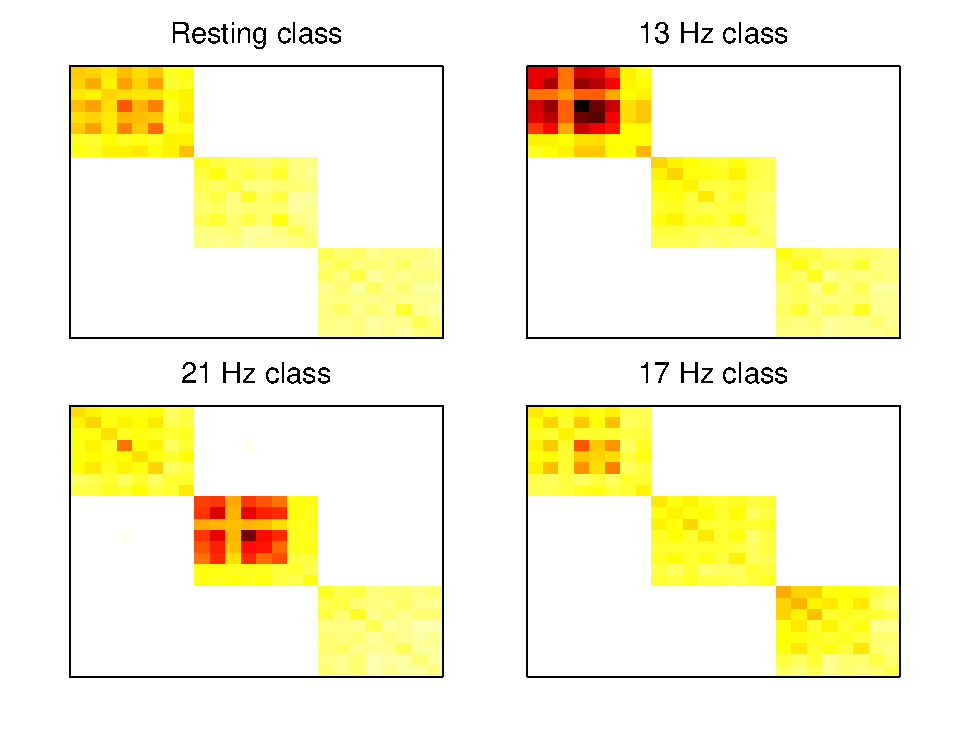
\includegraphics[width=0.47\textwidth]{Figures/covmat11.eps}
\label{fig:covmat11}}
\caption{Representation of covariance matrices: each image is the covariance matrix mean $\Pm^{(\ci)}$ of the class $\ci$, for one session of the recording. The diagonal blocks show the covariance in different frequency bands, i.e. 13Hz in the upper-left block, 21Hz in the middle, and 17Hz in the bottom-right. Subjects with highest (a) and lowest (b) BCI performance. 
}
\label{fig:covmat}
\end{figure}

% The MDM classifier is simple. Once the covariance matrices have been estimated, the only major calculations involved are the mean and distance computations.
The covariance matrices obtained from SSVEP data extended with Eq.~\eqref{eq:ext_data} have interesting features, allowing the discrimination between signals of identical sources but with different frequencies. 
Fig.~\ref{fig:covmat} shows the $K$ classes mean covariance matrices $\Pm^{(\ci)}$ from subjects with the highest (a) and lowest (b) classification accuracies. 
The three 8$\times$8 diagonal blocks hold the covariance matrices of the $\dF=3$ target frequencies.
Inter-frequencies covariances blocks are almost null.
In each mean covariance matrix, the block holding the covariance of the target frequency has the largest values. 
For the resting class, all $\dF$ blocks tend to have similar and small values. These features are more visible in the subject with the highest classification accuracy, and less visible in the one with lowest classification accuracy. 
It is interesting to see that features used for classification have a physiological meaning allowing an intuitive understanding, as opposed to \emph{black-boxes} approaches such as LDA or SVM. EEG processing complexity is encoded by the distance and not by machine learning.
% Contrary to discriminative classifiers classically used in BCI, such as LDA, SVM, etc, which appear as \emph{black-boxes} with difficult interpretation, it is very interesting to see that the presented covariance based classifier is based on features with an easy representation, and thus an intuitive understanding: the observed covariance matrices have a physiological meaning/interpretation.

Based on those covariance matrices, the different distances and means of Table~\ref{tab:dist} are compared in terms of classification accuracy and average CPU time elapsed on a trial classification, which involves the computation of 4 means of class and a distance to each mean.
Table~\ref{tab:res} summarizes results obtained for each subject and each distance/divergence.
Euclidean distance yields drastically low accuracy. 
This support the fact that using Euclidean distance and Arithmetic mean on SPD matrices is not appropriate. 
This is generally attributed to the invariance under inversion and the fact that the determinant of the Arithmetic mean of SPD matrices can be larger than the determinant of its parts; it is referred to as the \textit{swelling effect}.
Since the value of the determinant is a direct measure of dispersion of the multivariate variables (i.e. EEG channels and frequency bands), it leads to poor discrimination in the classification task. 
The swelling effect of Arithmetic mean is shown in Fig.~\ref{fig:swel}: the determinant of the Arithmetic mean is strictly larger than other means, the Log-Euclidean, Affine-Invariant and Bhattacharyya ones yielding similar determinants, close to trials values.

%\begin{sidewaystable}[t]
\begin{table*}[t]
\centering
%\ra{1}
\noindent\adjustbox{max width=\textwidth}{
\begin{tabular}{c|c|c|c|c|c|c||c|c|c|c|c|c|c|c|c|c|c|c|c|c|}
\cline{2-21}
& \multicolumn{6}{ c||}{Euclidean} & \multicolumn{14}{ c| }{Riemannian} \\ \cline{2-21}
& \multicolumn{2}{ c|}{Arithmetic}& \multicolumn{2}{ c|}{Harmonic}& \multicolumn{2}{ c||}{Geometric}&\multicolumn{2}{c|}{Log-Euclidean}&\multicolumn{2}{c|}{Affine-invariant}&\multicolumn{2}{c|}{$\alpha$-divergence}&\multicolumn{2}{c|}{Bhattacharyya}&\multicolumn{2}{c|}{Kullbacl-Leibler}&\multicolumn{2}{c|}{S-divergence}&\multicolumn{2}{c|}{Wassestein} \\ \cline{1-21}
\multicolumn{1}{ |c| }{Sub.} & acc (\%) & time(s)& acc (\%) & time(s)& acc (\%) & time(s)& acc (\%) & time(s)& acc (\%) & time(s)& acc (\%) & time(s)& acc (\%) & time(s)& acc (\%) & time(s) & acc (\%) & time(s) & acc (\%) & time(s)\\ \hline
\multicolumn{1}{ |c| }{1} & 53.12 & 0.025 & 48.44 & 0.015 & 00.00 & 0.000 & 71.88 & \textbf{0.150}& \textbf{73.44}& 0.194 & 			59.37 & 0.155 & 			68.75 & 			0.225 & 53.12 & 0.030 &  68.75  &  0.220  &  54.69  &  0.630\\ \hline
\multicolumn{1}{ |c| }{2} & 43.75 & 0.020 & 31.25 & 0.025 & 00.00 & 0.000 & 78.13 & 		0.160 & 			79.69 & 0.190 &			79.69 & 0.200 & \textbf{81.25} & \textbf{0.065} & 54.69 & 0.045 & 81.25  &  0.255  &  54.69  &  0.285\\ \hline
\multicolumn{1}{ |c| }{3} & 67.19 & 0.020 & 67.19 & 0.015 & 00.00 & 0.000 & 85.94 & 		0.120 &  		85.93 & 0.205 & \textbf{95.31} & 0.155 & 			85.94 & \textbf{0.100} & 71.88 & 0.060 & 85.94  &  0.200  &  76.56  &  0.280\\ \hline
\multicolumn{1}{ |c| }{4} & 54.68 & 0.030 & 42.19 & 0.010 & 00.00 & 0.000 & 84.38 & 		0.225 &  		87.50 & 0.315 & \textbf{89.07} & 0.250 & 			85.94 & \textbf{0.100} & 48.44 & 0.025 & 85.94  &  0.120  &  65.62  &  0.310\\ \hline
\multicolumn{1}{ |c| }{5} & 37.50 & 0.020 & 26.56 & 0.015 & 00.00 & 0.000 & 62.50 & \textbf{0.115}&  		68.75 & 0.290 & \textbf{73.44} & 0.140 & 			65.62 & 			0.125 & 67.19 & 0.030 & 65.63  &  0.110  &  45.31  &  0.660\\ \hline
\multicolumn{1}{ |c| }{6} & 34.37 & 0.015 & 39.06 & 0.020 & 00.00 & 0.000 & 84.38 & 		0.120 & 			85.94 & 0.210 & \textbf{87.50} & 0.145 & 			82.81 & \textbf{0.100} & 62.50 & 0.030 & 82.81  &  0.130  &  53.13  &  0.300\\ \hline
\multicolumn{1}{ |c| }{7} & 60.42 & 0.027 & 47.92 & 0.013 & 00.00 & 0.000 & 87.50 & 		0.267 &  		88.54 & 0.410 & \textbf{91.66} & 0.417 & 			86.46 & \textbf{0.137} & 54.17 & 0.043 & 86.46  &  0.243  &  69.79  &  0.777\\ \hline
\multicolumn{1}{ |c| }{8} & 67.19 & 0.035 & 68.75 & 0.015 & 00.00 & 0.000 & 90.63 & 		0.215 & \textbf{92.19} & 0.290 & \textbf{92.19} & 0.290 &  \textbf{92.19}& \textbf{0.125} & 71.88 & 0.050 & 92.19  &  0.165  &  85.94  &  0.335\\ \hline
\multicolumn{1}{ |c| }{9} & 57.81 & 0.035 & 42.19 & 0.015 & 00.00 & 0.000 & 70.31 &  		0.275 & 			70.31 & 0.380 & \textbf{75.00} & 0.300 & 			67.19 & \textbf{0.134} & 60.94 & 0.050 & 67.19  &  0.160  &  62.50  &  0.310\\ \hline
\multicolumn{1}{ |c| }{10} & 38.28 & 0.035 & 28.12 & 0.013 & 00.00 & 0.000 & 75.00 & 		0.254 & 			80.47 & 0.514 & \textbf{82.03} & 0.510 & 			78.13 & \textbf{0.160} & 67.97 & 0.028 & 78.13  &  0.263  &  51.56  &  0.650\\ \hline
\multicolumn{1}{ |c| }{11} & 48.44 & 0.025 & 46.88 & 0.010 & 00.00 & 0.000 & 60.94 & 		0.144 & 			65.63 & 0.235 & 			57.81 & 0.150 &  \textbf{75.00}& \textbf{0.105} & 39.06 & 0.040 & 75.00  &  0.195  &  56.25  &  0.575\\ \hline
\multicolumn{1}{ |c| }{12} & 71.25 & 0.032 & 53.75 & 0.022 & 00.00 & 0.000 & 96.25 & \textbf{0.292}& 		96.69 & 0.534 & 			95.62 & 0.634 &  \textbf{96.88} & 		0.300 & 76.88 & 0.042 & 96.88  &  0.466  &  82.50  &  1.042\\ \hline \hline
\multicolumn{1}{ |c| }{\textbf{Avg.}} & 52.83 & 0.027 & 45.19 & 0.016 & 00.00 & 0.000 & 78.98 & 0.194 & 81.27 & 0.314 & \textbf{81.56} & 0.279 & 80.51 & \textbf{0.140} & 60.72 & 0.039 & 80.51 &   0.210 & 63.21 & 0.513\\ \hline
\end{tabular}
}
\caption{Subject classification accuracies (acc(\%)) and average CPU time (time(s)) elapsed for the classification of a single trial. Classification is performed with MDM using either Euclidean or Riemannian means (see Table~\ref{tab:dist}).}
\label{tab:res}
\end{table*}
%\end{sidewaystable}

%\begin{sidewaystable}[t]
%%\begin{table*}[t]
%\centering
%%\ra{1}
%\begin{tabular}{c|c|c||c|c|c|c|c|c|c|c|}
%\cline{2-11}
%& \multicolumn{2}{ c||}{Euclidean} & \multicolumn{8}{ c| }{Riemannian} \\ \cline{2-11}
%& \multicolumn{2}{ c||}{Arithmetic}&\multicolumn{2}{c|}{Log-Euclidean}&\multicolumn{2}{c|}{Affine-invariant}&\multicolumn{2}{c|}{$\alpha$-divergence}&\multicolumn{2}{c|}{Bhattacharyya} \\ \cline{1-11}
%\multicolumn{1}{ |c| }{Sub.} & acc (\%) & time(s)& acc (\%) & time(s)& acc (\%) & time(s)& acc (\%) & time(s)& acc (\%) & time(s)\\ \hline
%\multicolumn{1}{ |c| }{1} & 53.12 & 0.025 & 71.88 & \textbf{0.150} & \textbf{73.44} & 0.194 & 59.37 & 0.155 & 68.75 & 0.225\\ \hline
%\multicolumn{1}{ |c| }{2} & 43.75 & 0.020 & 78.13 & 0.160 & 79.69 & 0.190 & 79.69 & 0.200 & \textbf{81.25} & \textbf{0.065}\\ \hline
%\multicolumn{1}{ |c| }{3} & 67.19 & 0.020 & 85.94 & 0.120 &  85.93 & 0.205 & \textbf{95.31} & 0.155 & 85.94 & \textbf{0.100}\\ \hline
%\multicolumn{1}{ |c| }{4} & 54.68 & 0.030 & 84.38 & 0.225 &  87.50 & 0.315 & \textbf{89.07} & 0.250 & 85.94 & \textbf{0.100}\\ \hline
%\multicolumn{1}{ |c| }{5} & 37.50 & 0.020 & 62.50 & \textbf{0.115} &  68.75 & 0.290 & \textbf{73.44} & 0.140 & 65.62 & 0.125\\ \hline
%\multicolumn{1}{ |c| }{6} & 34.37 & 0.015 & 84.38 & 0.120 & 85.94 & 0.210 & \textbf{87.50} & 0.145 & 82.81 & \textbf{0.100}\\ \hline
%\multicolumn{1}{ |c| }{7} & 60.42 & 0.027 & 87.50 & 0.267 &  88.54 & 0.410 & \textbf{91.66} & 0.417 & 86.46 & \textbf{0.137}\\ \hline
%\multicolumn{1}{ |c| }{8} & 67.19 & 0.035 & 90.63 & 0.215 & \textbf{92.19} & 0.290 & \textbf{92.19} &  0.290 & \textbf{92.19} & \textbf{0.125}\\ \hline
%\multicolumn{1}{ |c| }{9} & 57.81 & 0.035 & 70.31 &  0.275 & 70.31 & 0.380 & \textbf{75.00} & 0.300 & 67.19 & \textbf{0.134}\\ \hline
%\multicolumn{1}{ |c| }{10} & 38.28 & 0.035 & 75.00 & 0.254 & 80.47 & 0.514 & \textbf{82.03} & 0.510 & 78.13 & \textbf{0.160}\\ \hline
%\multicolumn{1}{ |c| }{11} & 48.44 & 0.025 & 60.94 & 0.144 & 65.63 & 0.235 & 57.81 & 0.150 & \textbf{75.00} & \textbf{0.105}\\ \hline
%\multicolumn{1}{ |c| }{12} & 71.25 & 0.032 & 96.25 & \textbf{0.292} & 96.69 & 0.534 & 95.62 & 0.634 & \textbf{96.88} & 0.300\\ \hline \hline
%\multicolumn{1}{ |c| }{\textbf{Avg.}} & 52.83 & 0.027 & 78.98 & 0.194 & 81.27 & 0.314 & \textbf{81.56} & 0.279 & 80.51 & \textbf{0.140}\\ \hline
%\end{tabular}
%\caption{Subject classification accuracies (acc(\%)) and average CPU time (time(s)) elapsed for the classification of a single trial. Classification is performed with MDM using either Euclidean or Riemannian means (see Table~\ref{tab:dist}).}
%\label{tab:res}
%%\end{table*}
%\end{sidewaystable}

\begin{figure}[h!]
\centering
\subfigure[]{
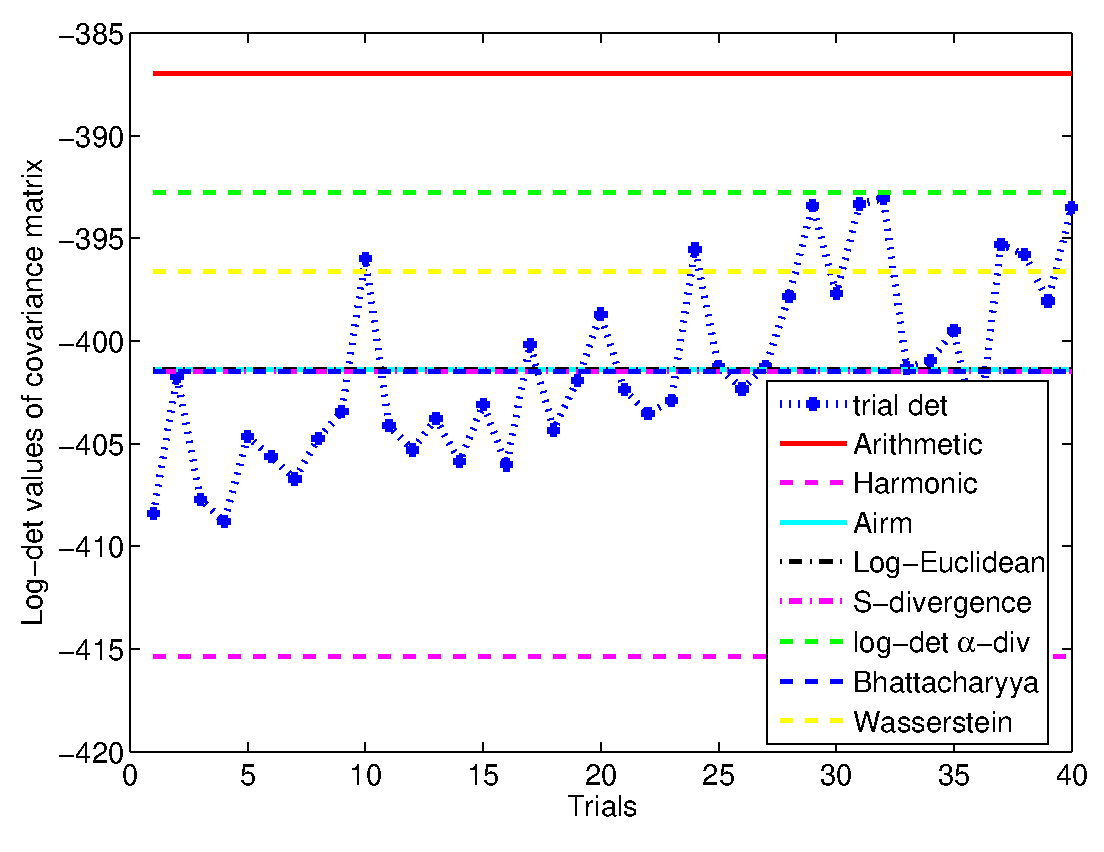
\includegraphics[width=0.46\textwidth]{Figures/swel.eps}
\label{fig:swel}
}
\subfigure[]{
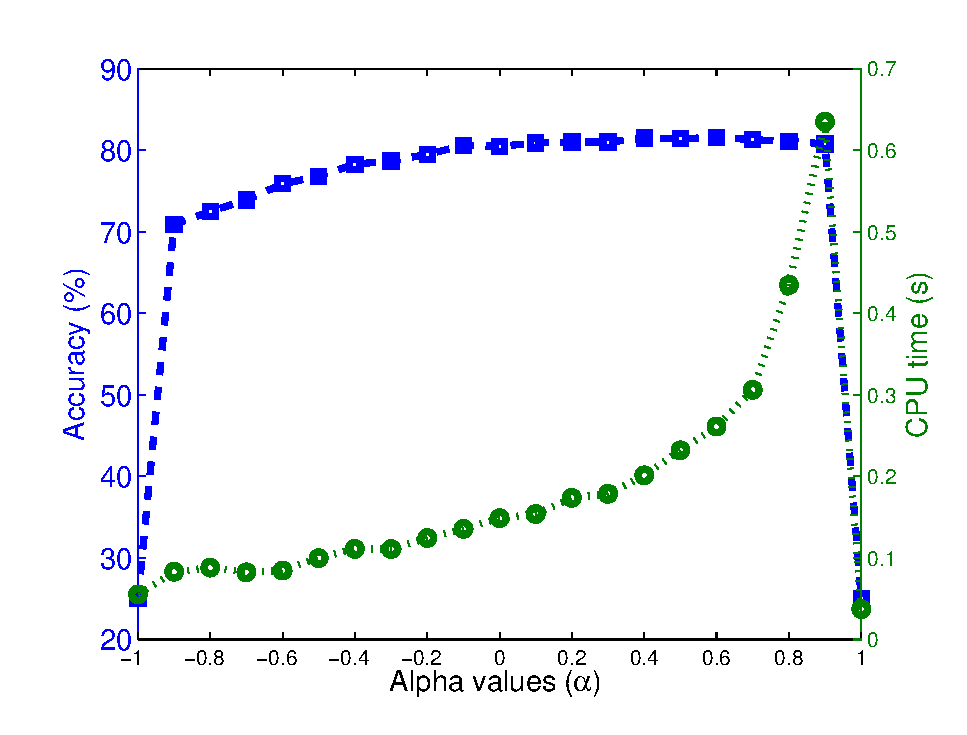
\includegraphics[width=0.49\textwidth]{Figures/alpha_cross.eps}
\label{fig:alphacross}
}
\caption{(a): Swelling effect of Arithmetic mean shown through log-determinant values. Training trials are taken from the 13Hz class of the subject with the highest BCI performance. Log-determinant values are given for each trial covariance (points), and for means of Table~\ref{tab:dist} (horizontal lines). (b): Classification accuracy and CPU time, obtained with $\alpha$-divergence for $-1\leqslant \alpha  \leqslant 1$.} 
\label{fig:swel_alpha}
\end{figure} 

Riemannian distances significantly improve classification performances, with $\alpha$-divergence yielding the best results (81.56\%). 
The value of $\alpha$ was set to 0.6 through cross-validation. 
This procedure lasted 225.42 seconds and makes $\alpha$-divergence the most costly method, due to the optimization of its parameter $\alpha$. 
Log-Euclidean yields lower classification accuracy (average 78.98\%) but could be computed faster than $\alpha$-divergence or Affine-Invariant distance.
However, the Bhattacharyya distance has the lowest computational cost of the considered Riemannian distances (average CPU time 0.140s), with a higher average accuracy of 80.51\%. 
So, it is good trade-off between efficiency and speed. 
The accuracies and CPU time of the $\alpha$-divergence at different values of $\alpha$ are shown in Fig.~\ref{fig:alphacross}.
It is seen that for $\alpha = \pm 1$, where $\alpha$-divergence represents a Bregman divergence associated with the log-determinant function, % also known as  log-det divergence, 
the classification accuracy are at the lowest accuracy (25\%). 
For all other values of alpha, the expected accuracy is 78.85$\pm$3.3\% and one can choose $-1 < \alpha < 1$ without any major impact on classification results.
%$\alpha$ could thus be fixed to any value between $\left]-1,+1\right[$ without causing drastic deterioration of accuracy. 
%For instance, the Bhattacharyya mean is equivalent to the $\alpha$-divergence mean with $\alpha$=0. 

This experiment on real EEG data shows that it is crucial to process covariance matrices with dedicated Riemannian tools, impacting the efficiency of the classification. 

%%%%%%%%%%%%%%%%%%%%%%%%%%%%%%%%%%%%%%%%%%%%%%%%%%%%%%%%%%%%%%%%%%%%%%%%%%%%%%%%

\section{Conclusion}
\label{sec:conclusion}

Riemannian approaches have been successfully applied on EEG signals for brain computer interfaces. 
Straightforward algorithms, such as Minimum Distance to Mean, provide competitive results with state-of-the-art methods, without requiring meticulous parametrization or optimization.
Working on covariance matrices in Riemannian spaces offers a wide choice of distances, embedding desirable invariances: it is thus possible to avoid the computation of user-specific spatial filters which are sensitive to artifacts and outliers.
Nonetheless, the estimation of the Riemannian geometric mean has a strong impact on the classifier accuracy.
This study investigates the performance of several distances and divergence on a real EEG dataset in the context of BCI based on the SSVEP paradigm.
The experimental results indicate that the $\alpha$-divergence yields the best accuracy after the selection of the best $\alpha$ values, but the Bhattacharyya distance has the lowest computational cost while providing honorable accuracies.

%%%%%%%%%%%%%%%%%%%%%%%%%%%%%%%%%%%%%%%%%%
\vspace{6pt} 

%%%%%%%%%%%%%%%%%%%%%%%%%%%%%%%%%%%%%%%%%%
%% optional
\supplementary{The following are available online at www.mdpi.com/link, Figure S1: title, Table S1: title, Video S1: title.}

%%%%%%%%%%%%%%%%%%%%%%%%%%%%%%%%%%%%%%%%%%
\acknowledgments{All sources of funding of the study should be disclosed. Please clearly indicate grants that you have received in support of your research work. Clearly state if you received funds for covering the costs to publish in open access.}

%%%%%%%%%%%%%%%%%%%%%%%%%%%%%%%%%%%%%%%%%%
\authorcontributions{For research articles with several authors, a short paragraph specifying their individual contributions must be provided. The following statements should be used ``X.X. and Y.Y. conceived and designed the experiments; X.X. performed the experiments; X.X. and Y.Y. analyzed the data; W.W. contributed reagents/materials/analysis tools; Y.Y. wrote the paper.'' Authorship must be limited to those who have contributed substantially to the work reported.}

%%%%%%%%%%%%%%%%%%%%%%%%%%%%%%%%%%%%%%%%%%
\conflictofinterests{Declare conflicts of interest or state ``The authors declare no conflict of interest.'' Authors must identify and declare any personal circumstances or interest that may be perceived as inappropriately influencing the representation or interpretation of reported research results. Any role of the funding sponsors in the design of the study; in the collection, analyses or interpretation of data; in the writing of the manuscript, or in the decision to publish the results must be declared in this section. If there is no role, please state ``The founding sponsors had no role in the design of the study; in the collection, analyses, or interpretation of data; in the writing of the manuscript, and in the decision to publish the results''.} 

%%%%%%%%%%%%%%%%%%%%%%%%%%%%%%%%%%%%%%%%%%
%% optional
%\abbreviations{The following abbreviations are used in this manuscript:\\
%
%\noindent MDPI: Multidisciplinary Digital Publishing Institute\\
%DOAJ: Directory of open access journals\\
%TLA: Three letter acronym\\
%LD: linear dichroism}
%
%%%%%%%%%%%%%%%%%%%%%%%%%%%%%%%%%%%%%%%%%%%
%%% optional
%\appendixtitles{no} %Leave argument "no" if all appendix headings stay EMPTY (then no dot is printed after "Appendix A"). If the appendix sections contain a heading then change the argument to "yes".
%\appendix
%\section{}
%The appendix is an optional section that can contain details and data supplemental to the main text. For example, explanations of experimental details that would disrupt the flow of the main text, but nonetheless remain crucial to understanding and reproducing the research shown; figures of replicates for experiments of which representative data is shown in the main text can be added here if brief, or as Supplementary data. Mathemtaical proofs of results not central to the paper can be added as an appendix.
%
%\section{}
%All appendix sections must be cited in the main text. In the appendixes, Figures, Tables, etc. should be labeled starting with `A', e.g., Figure A1, Figure A2, etc. 

%%%%%%%%%%%%%%%%%%%%%%%%%%%%%%%%%%%%%%%%%%
% Citations and References in Supplementary files are permitted provided that they also appear in the reference list here. 
\bibliographystyle{mdpi}

%%=====================================
%% References, variant A: internal bibliography
%%=====================================
%\renewcommand\bibname{References}
%\begin{thebibliography}{999}
%% Reference 1
%\bibitem{ref-journal}
%Lastname, F.; Author, T. The title of the cited article. {\em Journal Abbreviation} {\bf 2008}, {\em 10}, 142-149.
%% Reference 2
%\bibitem{ref-book}
%Lastname, F.F.; Author, T. The title of the cited contribution. In {\em The Book Title}; Editor, F., Meditor, A., Eds.; Publishing House: City, Country, 2007; pp. 32-58.
%\end{thebibliography}

%=====================================
% References, variant B: external bibliography
%=====================================
\bibliography{entropy}

%%%%%%%%%%%%%%%%%%%%%%%%%%%%%%%%%%%%%%%%%%
%% optional
%\sampleavailability{Samples of the compounds ...... are available from the authors.}

%%%%%%%%%%%%%%%%%%%%%%%%%%%%%%%%%%%%%%%%%%
\end{document}

\]